\begin{figure}[H]
  \centering
  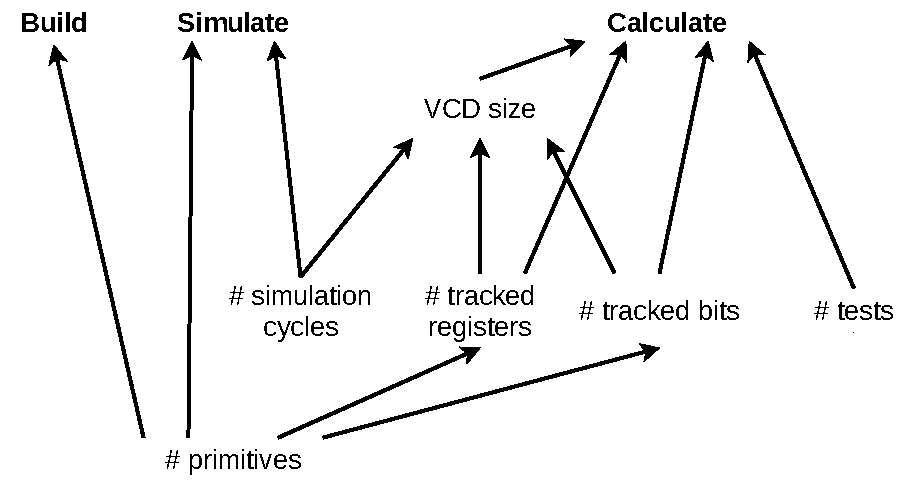
\includegraphics[width=0.81\textwidth,keepaspectratio]{../figures/evaluation/var-graph/var-graph.pdf}
  \caption{Directed-graph representation of \sysname{} software variables and
    their influence on the performance of the build, simulation, and calculate
    steps.}
  \label{fig:var-graph} 
\end{figure}

\begin{figure}[H]
  \centering
  \begin{subfigure}[T]{0.49\textwidth}
    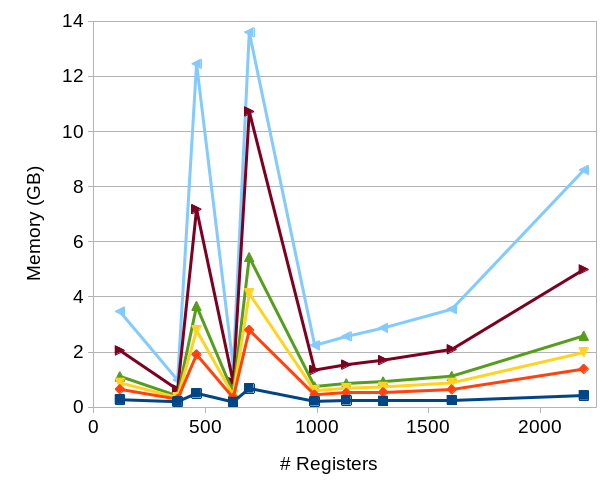
\includegraphics[width=\linewidth]{../figures/evaluation/calc-mem/cm-reg.png}
    \caption{}
    \label{fig:cm-reg}
  \end{subfigure}
  \begin{subfigure}[T]{0.49\textwidth}
    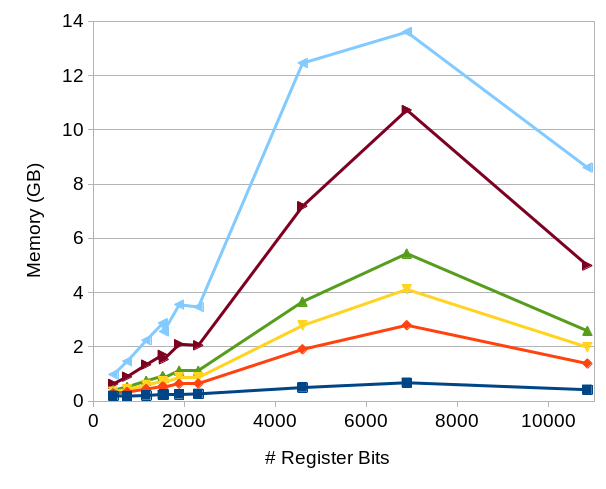
\includegraphics[width=\linewidth]{../figures/evaluation/calc-mem/cm-bit.png}
    \caption{}
    \label{fig:cm-bit}
  \end{subfigure}
  \begin{subfigure}[T]{0.49\textwidth}
    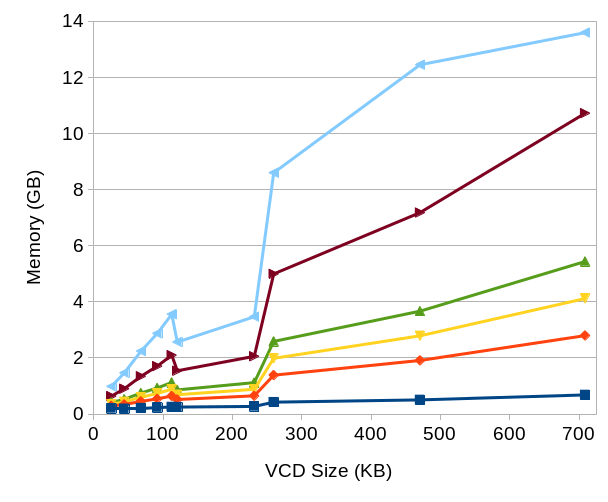
\includegraphics[width=\linewidth]{../figures/evaluation/calc-mem/cm-vcd.png}
    \caption{}
    \label{fig:cm-vcd}
  \end{subfigure}
  \begin{subfigure}[T]{0.49\textwidth}
    \parbox{\textwidth}{\centering\includegraphics[width=0.35\linewidth,frame]{../figures/evaluation/legend.png}}
    \label{fig:cm-legend}
  \end{subfigure}
  \caption{Calculation memory plotted as a function of (a) register count, (b)
    bit count and (c) VCD size.}
  \label{fig:calc-mem}
\end{figure}

\begin{singlespacing}
\begin{table}[H]
  \centering
  \caption{Resource usage of cryptographic FPGA cores used for testing
    \sysname{}'s performance.}
  \small
  \begin{tabular}{lrrrrrcrrr}
    \toprule

    % Organization
    &
    \multicolumn{5}{c}{Primitive Resources (\#)} &
    \phantom{} &
    \multicolumn{3}{c}{Sequential Signals} \\

    \cmidrule{2-6}
    \cmidrule{8-10}
    
    % Headings
    \multicolumn{1}{c}{\textbf{Name}} &
    \multicolumn{1}{c}{\textbf{LUT}} &
    \multicolumn{1}{>{\centering\arraybackslash}p{1.75cm}}{\textbf{Flip Flops}} &
    \multicolumn{1}{c}{\textbf{BRAM}} &
    \multicolumn{1}{c}{\textbf{DSP}} &
    \multicolumn{1}{c}{\textbf{Total}} &
    \phantom{} &
    \multicolumn{1}{c}{\textbf{Registers}} &
    \multicolumn{1}{>{\centering\arraybackslash}p{1.75cm}}{\textbf{Register Bits}} &
    \multicolumn{1}{>{\centering\arraybackslash}p{1.25cm}}{\textbf{Bits/ Reg.}} \\

    \midrule

    % Data
    \largeAES{} & 9612 & 10849 & -- & -- & 20461 && 2194 & 10848 & 4.944 \\
    \smallAES{} & 9031 & 1541 & -- & -- & 10572 && 1131 & 1540 & 1.362 \\
    \grycelAES{} & 539 & 592 & 16 & 18 & 1176 && 117 & 2298 & 19.641 \\
    \piedraDES{} & 382 & 307 & -- & -- & 691 && 375 & 430 & 1.147 \\

    \bottomrule
  \end{tabular}
  \label{tab:cores}
\end{table}
\end{singlespacing}

\begin{singlespacing}
\begin{table}[H]
  \centering
  \caption{Performance benchmarks for the simulate step for different designs
    when only analyzing one secret input bit.}
  \small
  \begin{tabular}{rrrrcrcrr}
    \toprule

    % Organization
    \multicolumn{4}{c}{Analysis Parameters (\#)} & \phantom{} & \phantom{} & \phantom{a} & \multicolumn{2}{c}{Performance Metrics} \\

    \cmidrule{1-4}
    \cmidrule{8-9}
    
    % Headings
    \multicolumn{1}{c}{\textbf{Primitives}} &
    \multicolumn{1}{c}{\textbf{Registers}} &
    \multicolumn{1}{>{\centering\arraybackslash}p{2cm}}{\textbf{Register Bits}} &
    \multicolumn{1}{c}{\textbf{Cycles}} &
    &
    \multicolumn{1}{c}{\textbf{\# Tests}} &
    &
    \multicolumn{1}{>{\centering\arraybackslash}p{2cm}}{\textbf{Peak Memory}} &
    \multicolumn{1}{>{\centering\arraybackslash}p{1.75cm}}{\textbf{Runtime}} \\

    % Units
    & & & & & & & \multicolumn{1}{c}{(GB)} & \multicolumn{1}{c}{(seconds)} \\

    \midrule

    % Data
    20461 & 2194 & 10848 & 44 && 50 && 1.632476 & 784.61 \\
                          &&&&& 250 && 2.459708 & 1089.59 \\
                          &&&&& 375 && 3.620812 & 1274.37 \\
                          &&&&& 500 && 4.781652 & 1486.3 \\
    \midrule
    10572 & 1131 & 1540 & 91 && 50 && 1.53916 & 186.68 \\
                          &&&&& 250 && 1.736008 & 387.36 \\
                          &&&&& 375 && 2.552068 & 519.23 \\
                          &&&&& 500 && 3.370008 & 642.07 \\
    \midrule
    1176 & 117 & 2298 & 251 && 50 && 1.494316 & 75.65 \\
                          &&&&& 250 && 1.487516 & 241.72 \\
                          &&&&& 375 && 1.491108 & 351.54 \\
                          &&&&& 500 && 1.743848 & 470.87 \\
    \midrule
    691 & 375 & 430 & 16 && 50 && 1.499956 & 37.29 \\
                          &&&&& 250 && 1.50056 & 56.99 \\
                          &&&&& 375 && 1.500296 & 70.78 \\
                          &&&&& 500 && 1.49832 & 84.35 \\
    \bottomrule
  \end{tabular}
  \label{tab:bench-sim}
\end{table}
\end{singlespacing}

\begin{singlespacing}
\begin{minipage}[H]{0.83\textwidth}
\begin{algorithm}[H]
  \label{alg:sheila}
  \caption{\small Process for generating, collecting, and processing data to
    determine leakage scores for all device registers.}

  \KwIn{$K$ = set of secret bits to test}
  \KwIn{$R$ = set of registers to analyze}
  \KwIn{$m$ = number of clock cycles to simulate device}
  \KwIn{$n$ = number of simulations per bit polarity}
  \KwOut{$L$ = set of leakage scores for all registers}

  \For{$k \in K$}{
    \For{$i \leftarrow 0$ \KwTo $n-1$}{
      Randomize all inputs\;
      $k \leftarrow 0$\;
      $\textbf{S} \leftarrow$ SimulateDevice($m$)\;
      \For{$r \in R$}{
        trace$_{r0i} \leftarrow \{(r,v)_{t}) \in \textbf{S} \mid 0 < t < m\}$
      }
    }
    \For{$i \leftarrow 0$ \KwTo $n-1$}{
      Randomize all inputs\;
      $k \leftarrow 1$\;
      $\textbf{S} \leftarrow$ SimulateDevice($m$)\;
      \For{$r \in R$}{
        trace$_{r1i} \leftarrow \{(r,v)_{t}) \in \textbf{S} \mid 0 < t < m\}$
      }
    }
    \For{$r \in R$}{
      SecretDist $\leftarrow \overrightarrow{0}||\overrightarrow{1}$\;
      TraceDist$_{0} \leftarrow$ trace$_{r00} |$trace$_{r01} | ... |$trace$_{r0n-1}$\;
      TraceDist$_{1} \leftarrow$ trace$_{r10} |$trace$_{r11} | ... |$trace$_{r1n-1}$\;
      $l \leftarrow MI($SecretDist, TraceDist$_{0} || $TraceDist$_{1})$\;
      $L$ append $(r,l)$\;
    }
  }
\end{algorithm}
\end{minipage}
\end{singlespacing}

\begin{lstlisting}[xleftmargin=0.01\textwidth,
  caption={Sample database entry for one device register, showing all device
    nets that comprise the register and its leakage scores for different secret
    input bits.},
  label=lst:db, float=!ht, language=json]
{
    "sim_name": "/sheila_tb/uut/aes_datapath_inst/mix_cols_inst/low_bits_dsp_in_3",
    "num_nets": "8",
    "net_list": [
      "aes_datapath_inst/mix_cols_inst/low_bits_dsp_in_3[16]",
      "aes_datapath_inst/mix_cols_inst/low_bits_dsp_in_3[17]",
      "aes_datapath_inst/mix_cols_inst/low_bits_dsp_in_3[18]",
      "aes_datapath_inst/mix_cols_inst/low_bits_dsp_in_3[19]",
      "aes_datapath_inst/mix_cols_inst/low_bits_dsp_in_3[20]",
      "aes_datapath_inst/mix_cols_inst/low_bits_dsp_in_3[21]",
      "aes_datapath_inst/mix_cols_inst/low_bits_dsp_in_3[22]",
      "aes_datapath_inst/mix_cols_inst/low_bits_dsp_in_3[23]",
    ],
    "num_secrets": 5,
    "scores": [
      0.06049263993130438,
      0.061025747257136276,
      0.05185308240550879,
      0.05146929700615743,
      0.057104940634903345,
    ],
    "color": "{255 243 179}"
  },
\end{lstlisting}